\documentclass{article}
\usepackage{xcolor}
\usepackage{url}
\usepackage{hyperref}
\usepackage{graphicx}
\usepackage{soul}
\usepackage{enumerate}
\usepackage{fancyhdr}
\usepackage{listings}

% Define custom colors
\definecolor{bg}{rgb}{0.64, 0.64, 0.82}
\definecolor{frame}{rgb}{0.59, 0.47, 0.71}
\definecolor{keyword}{rgb}{0.63, 0.36, 0.94}
\definecolor{comment}{rgb}{0.44, 0.5, 0.56}
\definecolor{string}{rgb}{0.56, 0.27, 0.52}

% Set custom listings options
\lstset{
    backgroundcolor=\color{bg},
    frame=single,
    rulecolor=\color{frame},
    basicstyle=\ttfamily\small,
    keywordstyle=\color{keyword}\bfseries,
    commentstyle=\color{comment},
    stringstyle=\color{string},
    showstringspaces=false,
    breaklines=true,
    xleftmargin=2mm,
    xrightmargin=2mm
}
% Header
\pagestyle{fancy}
\fancyhf{}
\fancyhead[L]{MAD 102 - Intro to Prog - Fall 2024}
\fancyhead[R]{Instructor: Aishwarya Rajasekaran \thepage}

\title{Looping - MAD 102 Week 4 Notes}
\author{Hia Al Saleh}
\date{September 18th, 2024}
\begin{document}
\maketitle
\tableofcontents 
\newpage
\section{Looping and Repetition Structures}
In programming, repetition structures, also known as loops, are used to execute the same section of code multiple times. This is particularly useful when you want to repeat the same task without duplicating your code, following the DRY principle (Don’t Repeat Yourself).

\subsection{Advantages of Loops}
Loops offer several advantages, including:
\begin{itemize}
    \item Efficient use of a single set of instructions to process multiple data sets.
    \item Flexibility to incorporate selection structures, allowing varied treatments of different data based on conditions.
    \item Ability to operate on known or unknown quantities of data.
\end{itemize}

\subsection{Components of a Loop}
A loop has three critical components:
\begin{enumerate}
    \item \textbf{Initialization}: Assign an initial value to the loop variable.
    \item \textbf{Condition Evaluation}: Determine whether the loop should continue based on a conditional expression.
    \item \textbf{Alteration}: Modify the loop variable so that the condition will eventually be false, preventing infinite loops.
\end{enumerate}

\section{While Loops}
A \textbf{while loop} executes as long as a specified condition is true. It's a pretest loop, meaning the condition is tested before the loop body is executed.

\begin{lstlisting}[language=python]
loop_variable =1
while loop_variable <= 3:
  print("loop executed")
  print(f"Lteration:{loop_variable}")
  loop_variable = loop_variable +3

print("loop finished")
\end{lstlisting}

\subsection{For Loops}
A \textbf{for loop} is commonly used to iterate over a sequence or container (like a list). No sentinel value is required; the loop runs as many times as there are items in the container.

\begin{lstlisting}[language=python]
list_strings = ['Apple', 'Pear', 'Mango']
for string in list_strings:
    print(string)
\end{lstlisting}

\subsection{Using Ranges in For Loops}
The \texttt{range()} function allows you to generate a sequence of numbers within a loop.
\begin{lstlisting}[language=python]
for i in range(5):
    print(i)
for i in range(15, 5, -3):
    print(i)
\end{lstlisting}
\subsection{Ranges}
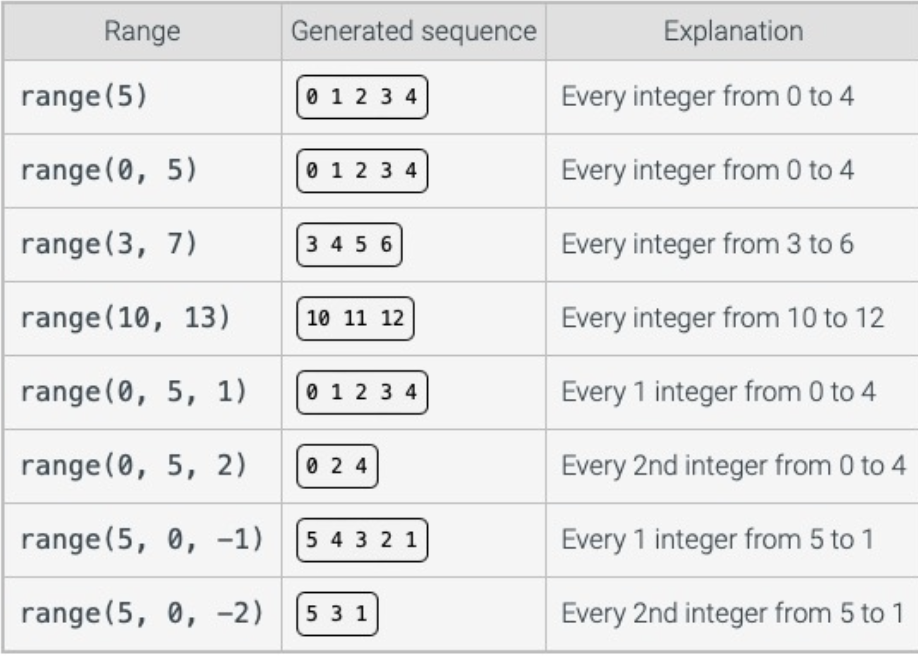
\includegraphics[width=11.5cm]{Lecture_Notes_In_LaTex/imgs/ranges.png}

\subsection{Savings Calculation Example}

\begin{lstlisting}[language=Python]
initial_savings = 200
interest_rate = 0.05

years = int(input('Enter years: '))
print()

savings = initial_savings
for i in range(years):
    print(f'Savings in year {i}: ${savings:.2f}')
    savings += savings * interest_rate

\end{lstlisting}

\subsection{Nested Loops}
A \textbf{nested loop} is a loop within another loop. The inner loop completes all its iterations for every single iteration of the outer loop.

\begin{lstlisting}[language=Python]
for hours in range(1):
    for minutes in range(60):
        for seconds in range(60):
            print(f'{hours}:{minutes}:{seconds}')
\end{lstlisting}
\section{Break and Continue Statements}
The \texttt{break} statement allows you to exit a loop prematurely, while the \texttt{continue} statement skips the rest of the code in the loop and proceeds to the next iteration.

\subsection{Break Statement Example}

\begin{lstlisting}[language=Python]
for number in range(1, 101):
    if number % 2 == 1:
        break
    print('This will never run')
\end{lstlisting}
\begin{enumerate}
    \item The break statement is used to immediately exit a loop
    \item If I want to display the numbers from 1 – 100 that are even, I could use this code.
\end{enumerate}

 
\subsection{Continue Statement Example}

\begin{lstlisting}[language=Python]
for number in range(1, 101):
    if number == 5:
        continue
    print(f'{number} is an even number')
\end{lstlisting}

\section{Enumerate Function}
Sometimes you need both the index and the value of elements in a collection. The \texttt{enumerate()} function creates a tuple with the index and value, allowing easy access to both.

\begin{lstlisting}[language=Python]
students = ["Mal", "Simon", "Zoe", "River"]

for (index, student) in enumerate(students):
    print(f'{student} is located at index {index}')
\end{lstlisting}

\section{Exercises}

\subsection{Exercise 1}
We want to create a program that will add two numbers together and return the result. Unlike previous exercises, we will continue to ask the user for numbers until they no longer want to use our program.
\subsection*{Solution}
\begin{lstlisting}[language=Python]
user_choice_to_continue = 'Y'
while user_choice_to_continue == 'Y':
    num1 = int(input('Please enter your first number: '))
    num2 = int(input('Please enter your second number: '))
    sum_result = num1 + num2
    print(f'The sum of {num1} + {num2} = {sum_result}')
    
    user_choice_to_continue = input('Would you like to continue? Y/N: ').upper()
    if user_choice_to_continue not in ['Y', 'N']:
        user_choice_to_continue = input('Invalid input. Please enter Y or N: ')
\end{lstlisting}

\subsection{Exercise 2}
Create a program that will count down from a specific number to 0.
\subsection*{Solution}
\begin{lstlisting}[language=python]
# introduce the program
print('It\'s a countdown!')
print('==' * 30)
number = int(input('Please enter a number to countdown from:'))
# display the results
print(f'Counting down from {number}:')
while number > -1:
  print(number)
  number -= 1
# end of program
print('Your Program Ends here!')
\end{lstlisting}
\subsection{Exercise 3}
Create a countdown program that will count down to 0 from a provided minute value Display the results to the screen
\subsection*{Solution}
\begin{lstlisting}[language=python]
# declare variables
second = 59 
# introduce the program 
print('It\'s a countdown!') 
print('=='*30) 
minute = int(input('Please enter a minute to countdown from:')) 
# display the results 
print(f'Counting down from {minute}:') 

while minute >=0:
  while second >=0:
    print(f'{minute}:{second}')
    second -=1 
  minute -= 1
  second = 59
# end of program 
print('Blast off!')
\end{lstlisting}
\subsection{Exercise 4}
We want to keep track of our grocery purchases for a day. We then want to know how much we spent. Some days we may not enter anything – so it should display no amount was spent. The purchases vary from day to day
\subsection*{Solution}
\begin{lstlisting}[language=python]
# Declare variables
purchases = []  # Initialize a list to store purchases
total_amount_spent = 0  # Initialize total amount spent

# Introduce Program
print("Welcome to the Grocery Purchase Tracker!")

# Initial user input
purchased = input("Did you purchase any grocery items today ('yes' or 'no'): ").strip().lower()

# Keep prompting the user for purchases until they choose to stop
while True:
    if purchased != "yes" and purchased != "no":
        purchased = input("Enter valid input ('yes' or 'no'): ").strip().lower()
    
    if purchased == 'no':
        break
    elif purchased == 'yes':
        item = input("Enter item name: ")
        
        while True:
            try:
                price = float(input("Enter the price of the item: $"))
                break  # Exit the loop if the price is valid
            except ValueError:
                print("Invalid price. Please enter a valid number.")
        
        purchases.append((item, price))  # Add the item and price to the list of purchases
        total_amount_spent += price  # Update total amount spent
        # Ask if more purchases are made
        purchased = input("Did you purchase more grocery items today ('yes' or 'no'): ").strip().lower()
# Display the purchases and total amount spent
if purchases:
    print("\nYour purchases for the day:")
    for item, price in purchases:
        print(f"{item}: ${price:.2f}")
    print(f"\nTotal amount spent for the day: ${total_amount_spent:.2f}")
else:
    print("\nNo purchases were made today. No amount was spent.")
# Sample additional loop example (adjusted)
for i, s in enumerate(range(1, 5)):
    print("index", i)
    print(s)
    
\end{lstlisting}
\end{document}